\section{Dual topology monitoring}
\label{section:complete-igp}

As we showed before, the minimum number of segments required to cover a topology can be quite high.
One idea to reduce it is to have a separate set of IGP weights. The ones already configured on the network used
to forward traffic and new ones that are used only for sending the monitoring probes.

One idea to compute those weights would be to first compute a minimum cycle cover of the network using
some standard existing algorithm \cite{FAN1992113} (note that here we are talking about cycles, not 
sr-cycles). Then we could compute a set of weights such that the maximum number of segments required to
segment any of those cycles is as small as possible. We did not solve this problem and therefore leave
it as an open problem (with a slightly more general formulation).

\begin{problem}{Optimal segmentation IGP}
Given a graph $G$ and a set $P$ of paths on $G$ compute a IGP weight function 
$\igp : E(G) \rightarrow \mathbb{N}$ such that if we compute a minimal segmentation
of every path $p \in P$ whose maximum segment cost amongst those sr-paths is minimal.
\end{problem}

We believe that solving this problem could be very useful in any setting where having a dual weight
topology is infeasible in practice. This would be yet another way to leverage existing graph theory to solve the 
problem and then translate those graph theoretic solutions into segment routing solutions with low
segment cost.

Another possibility, which we explore in this thesis, is to compute a set of $\igp$ weights such that 
there is a unique shortest path between any pair of nodes \emph{and} every edge belongs to a unique shortest
path. The intuition of why this will make segmentations less costly is that the conditions for needing to add
a new segment in the minimum segmentation algorithm is exactly the existence of multiple shortest paths or
an edge that does not belong to any shortest path.
Note that our two conditions cannot both coexist in a network with parallel links. With two links between
$u$ and $v$, we cannot have at the same time that both those links belong to some shortest path and a unique
shortest path between $u$ and $v$. We therefore relax the definition as follows.

\begin{definition}
Let $G$ be a graph. A set of IGP weights $\igp : E(G) \rightarrow \mathbb{N}$ is said to be
\emph{complete} if and only if for all $u, v \in V(G)$ at least one edge of $E(G, u, v)$ belong to a shortest path.
\end{definition}

\begin{definition}
Let $G$ be a graph. A set of IGP weights $\igp : E(G) \rightarrow \mathbb{N}$ is said to be
\emph{ECMP-free} if and only if for all $u, v \in V(G)$ there is a unique shortest path between $u$ and $v$.
\end{definition}

\subsection{Computing ECMP-free and complete IGP weights}

\begin{definition}
Let $G$ be a graph. A set of IGP weights $\igp : E(G) \rightarrow \mathbb{N}$ is said to be
\emph{total} if and only all simple paths on $G$ have a different weight.
\end{definition}

Computing a total weighting of a graph $G$ is trivial. We can simply set $\igp(e) = 2^{\idx(e)}$ for
all $e \in E(G)$. Since $\idx(e)$ assigns a unique index between $0$ and $|E(G)| - 1$ to the edges
of $G$, this IGP function will assign a different power of two to each edge of $G$. Therefore,
any two distinct simple paths must have a different IGP weight since those weights will
correspond to sums of distinct powers of $2$.

The following lemma shows, unsurprisingly, that one way to build ECMP-free weights is to compute
total weights.

\begin{lemma}
\label{lemma:totalToECMP}
Let $G$ be a graph. If $\igp : E(G) \rightarrow \mathbb{N}$ is total then it is ECMP-free.
\end{lemma}

\begin{proof}
Trivial from the definition. Any shortest path is simple and thus any two shortest paths must 
have a different IGP weight since $\igp$ is total.
\end{proof}

The following result shows that we can transform any total IGP weighting $\igp$ into a complete one by
adding a large enough constant. This constant can by any value above the maximum between the diameter of the
graph with respect to $\igp$ and the maximum weight of any edge. Being larger than the diameter ensures
that shortest paths remain unique and being larger than the maximum weight ensures that every edge belong to a shortest path. 
The diameter of a network is the greatest distance (in terms of number of edges)
between any pair of vertices.

\begin{lemma}
\label{lemma:totalToComplete}
Let $G$ be a network. Let 
$$
M \geq \max \left( diam(G, \igp), \displaystyle \max_{e \in E(G)} \igp(e) \right).
$$
Then, if $\igp : E(G) \rightarrow \mathbb{N}$ is total then 
$\igp^+ : E(G) \rightarrow \mathbb{N}$ defined by $\igp^+(e) = \igp(e) + M$ is complete.
\end{lemma}

\begin{proof}
Let $p_1 = (e_1, \ldots, e_n)$ and $p_2 = (f_1, \ldots, f_m)$ be two paths on $G$. 

We start by proving that $\igp^+(p_1) \neq \igp^+(p_2)$. By definition
$\igp^+(p_1) = \igp(p_1) + n \cdot M$ and $\igp^+(p_2) = \igp(p_2) + m \cdot M$. By hypothesis, 
$\igp(p_1) \neq \igp(p_2)$ Assume without loss of generality that $\igp(p_1) > \igp(p_2)$. If $n = m$ then
\begin{align*}
\igp^+(p_1) = \igp(p_1) + n \cdot M > \igp(p_2) + n \cdot M = \igp(p_2) + m \cdot M = \igp^+(p_2).
\end{align*}
By definition of $M$, we have $M \geq diam(G, \igp) \geq \igp(p_1), \igp(p_2) > 0$. Thus, if $n > m$ then,
\begin{align*}
\igp^+(p_1) & = \igp(p_1) + n \cdot M > n \cdot M \geq (m + 1) \cdot M \\
& = M + m \cdot M \geq \igp(p_2) + m \cdot M = \igp^+(p_2)
\end{align*}
Similarly, if $n < m$ then
\begin{align*}
\igp^+(p_2) & = \igp(p_2) + m \cdot M > m \cdot M \geq (n + 1) \cdot M \\
& = M + n \cdot M \geq \igp(p_1) + n \cdot M = \igp^+(p_1).
\end{align*}
Thus, in any case, $\igp^+(p_1) \neq \igp^+(p_2)$. We conclude that $\igp^+$ is total
and therefore also ECMP-free.

Let $u, v \in V(G)$. We now show that at least one edge $e \in E(G, u, v)$ belongs to a shortest path with respect to $\igp^+$.
Let $e \in E(G, u, v)$ be such that $\igp(e)$ is minimum. Since $\igp$ is total, this edge is unique. 
By Proposition \ref{prop:sp-properties}, $e$ belongs to a shortest path if and only if $e$ is a shortest path between
$u$ and $v$. Suppose that $e$ is not a shortest path for $\igp^+$. Then there exists a path $p = (e_1, \ldots, e_n)$ from $u$ to $v$ such that
$\igp^+(p) < \igp(e)$. Since $e$ is the unique edge between $u$ and $v$ of minimum cost, $n \geq 2$. By definition of $M$, we have $M \geq \igp(e)$ so 
\begin{align*}
\igp^+(p) = \igp(p) + n \cdot M \geq \igp(p) + 2 \cdot M > 2 \cdot M \geq 2 \cdot \igp(e) > \igp(e).
\end{align*}
This contradicts the fact that $e$ is not a shortest path for $\igp^+$. Therefore $\igp^+$ is complete.
\end{proof}

\begin{corollary}
Let $G$ be a graph and $\igp : E(G) \rightarrow \mathbb{N}$ defined such that
$$
\igp(e) = 2^{\idx(e)} + 2^{|E(G)|}.
$$
Then $\igp$ is ECMP-free and complete.
\end{corollary}

\begin{proof}
We have already observed that $e \mapsto 2^{\idx(e)}$ is total and thus ECMP-free by Lemma \ref{lemma:totalToECMP}. Completeness then follows from
Lemma \ref{lemma:totalToComplete} by observing that 
$$
2^{|E(G)|} = \left( \sum_{e \in E(G)} 2^{\idx(e)} \right) + 1 > \max \left( diam(G, \igp), \displaystyle \max_{e \in E(G)} \igp(e) \right).
$$
\end{proof}

The problem with these IGP weights is that they are exponential with respect to the number of edges in the graph.
In practice IGP weights are represented with a $16$-bit integer and thus is maximum value is $2^{16} - 1 = 65535$.
This makes them useless in practice since they can only be implemented on a network with at most $15$ edges.

This motivates the following problem.

\begin{problem}{Minimum weight complete weighting}
\label{prob:minComplete}
\textbf{Input:} A network $G$.

\textbf{Output:} A complete and ECMP-free weighting $\igp : E(G) \rightarrow \mathbb{N}$ such that
$\displaystyle \max_{e \in E(G)} \igp(e)$ is minimum.
\end{problem}

Any approach for solving Problem \ref{prob:minComplete} that is based on Lemma \ref{lemma:totalToComplete} is domed to fail.
To see why this is true consider $\mathcal{K}_n$, the complete graph on $n$ nodes. It is not hard to see that $\mathcal{K}_n$ 
contains an exponential number of simple paths. 

%Any simple path on $\mathcal{K}_n$ corresponds to a sequence of nodes
%of length at most $n - 1$ without repetitions. Therefore, the number of such paths is
%$$
%P = \frac{1}{2} \sum_{l = 2}^n \frac{n!}{(n - l)!} \approx \frac{en!}{2}.
%$$

Any permutation of $n$ elements corresponds to a simple path on $\mathcal{K}_n$ 
of length $n - 1$ and there are $n!$ permutations of $n$ elements. Since a total weight must assign a different weight to
\emph{every} simple path, this shows that a total weight on the complete graph $\mathcal{K}_n$ will be such that at least
one simple path of length $n - 1$ has a weight of at least $n!$. Therefore this path must contain one edge of weight
$\frac{n!}{n - 1}$ since otherwise the total weight of the path would be lower than $n!$.

This shows that total weightings require exponential weights on any graph with an exponential number of paths. Most graphs
have an exponential number of simple paths with respect to its size. Hence, using Lemma \ref{lemma:totalToComplete} is bound
to provide weights that are very high. In contrast, it is not hard to see that $e \mapsto 1$ is an ECMP-free and complete weighting of
$\mathcal{K}_n$. This shows that such exponential bounds do not apply for the weight that we are looking for, only for total ones.

If we only care about the practical applicability of the weights, we can relax Problem \ref{prob:minComplete} into the following one.

\begin{problem}{Implementable complete weighting}
\label{prob:implemComplete}
\textbf{Input:} A network $G$.

\textbf{Output:} A complete and ECMP-free weighting $\igp : E(G) \rightarrow \mathbb{N}$ such that
$\displaystyle \max_{e \in E(G)} \igp(e) \leq 2^{16} - 1$.
\end{problem}

\subsection{Prime-based complete IGP}

We propose a partial solution to Problem \ref{prob:implemComplete}. Our solution is able to find a solution for $97.7\%$ of the instances in our dataset.
Let $m = |E(G)|$ be the number of edges in the graph and $\mathbb{P}_m = \{ \pi_0, \ldots, \pi_{m - 1} \}$ a set of $m$ prime numbers such that
$\pi_i \leq \pi_{i + 1}$. It is well known that two sets of distinct prime numbers
have a different product. Our idea is based on the fact that $\log(x \cdot y) = \log(x) \cdot \log(y)$. If we could set any real valued IGP weights,
one solution would be to use $e \mapsto \log(\pi_{\idx(e)})$ because the unicity of products between prime numbers would translate into unique sums
and thus unique path weights. To simplify the notations, we write $\pi_e$ instead of $\pi_{\idx(e)}$.
In this way, by what we observe above, two distinct paths would necessarily have distinct IGP costs.

Since we need integers we will use truncated logarithms instead. These logarithms are defined as
$$
\lnt{s}(x) = \lfloor 10^s \cdot \ln(x) \rfloor.
$$
For instance, $\lnt{4}(5) = \lfloor 10^4 \cdot 1.60943 \rfloor = 16094$. The idea is, starting from $s = 1$, to grow $s$ 
until the IGP weights defined by $e \mapsto \lnt{s}(\pi_e)$ are ECMP-free. A priori, nothing guarantees that doing so will 
eventually achieve it but we will prove shortly that it does. Since we also want the IGP weights to also be complete, we use
a slight different set of IGP weights $\igp^s : E(G) \rightarrow \mathbb{N}$ defined as $\igp^s(e) = \lnt{s}(\pi_e) + \lnt{s}(\pi_m)$.
The intuition behind the addition of the largest $\lnt{s}(\pi_m)$ term for achieving completeness is similar to the addition of the constant $M$
from Lemma \ref{lemma:totalToComplete}. We now prove that by growing $s$, $\igp^s$ eventually becomes ECMP-free and complete.

  
\begin{proposition}
\label{prop:converge}
Let $A$ and $B$ be two distinct subsets of $\mathcal{P}_m$, $P = \prod_{x \in \mathcal{P}_x} x$ and $q \in \mathcal{P}_m$. If $s > \log_{10} \left( 2 m \cdot q^m P \right)$, 
then 
$$
\sum_{x \in A} \left( \overline{\ln}^s(x) + \overline{\ln}^s(q) \right) \neq \sum_{x \in B} \left( \overline{\ln}^s(x) + \overline{\ln}^s(q) \right).
$$
\end{proposition}

\begin{proof}
Given any $s$ and $X \subseteq \mathcal{P}_m$, we have
\begin{equation}
\small
\label{eq:lg}
10^s \cdot \ln \left( \prod_{x \in X} x \right) \geq \sum_{x \in X} \overline{\ln}^s(x) \geq 10^s \cdot \ln \left( \prod_{x \in X} x \right) - |X|
\end{equation}

Let $q \in \mathcal{P}_m$. Write $a = \prod_{x \in A} x$ and $b = \prod_{x \in B} x$. Assume without loss of generality that $q^{|A|} a > q^{|B|} b$ (they are not equal because they contain distinct prime numbers). 
Then by (\ref{eq:lg})
\begin{align*}
\tiny
\sum_{x \in A} \overline{\ln}^s(x) +  \overline{\ln}^s(q) & \geq \sum_{x \in A} 10^s \ln(x q) - 2 \geq \\
& 10^s \ln(q^{|A|} a) - 2 |A|
\end{align*}
and $\sum_{x \in B} \overline{\ln}^s(x) + \overline{\ln}^s(q) \leq 10^s \ln (q^{|B|} b)$. Therefore
\begin{align*}
\tiny
\sum_{x \in A} \overline{\ln}^s(x) +  \overline{\ln}^s(q) - \sum_{x \in B} \overline{\ln}^s(x) + \overline{\ln}^s(q) & \geq \\
10^s \ln(q^{|A|} a) - 2 |A| - 10^s \ln (q^{|B|} b) & \geq \\
10^s  \ln \left(q^{|A|} a \slash q^{|B|} b \right) - 2 |A| \geq & \\
10^s  \ln \left(q^{|A|} a \slash (q^{|A|} a - 1) \right) - 2 |A| \geq & \\
10^s \slash (q^{|A|} a) - 2|A| \geq 10^s \slash (q^m P) - 2m
\end{align*}
Which is positive as long as $s > \log_{10} \left( 2 m \cdot q^m P \right)$.
\end{proof}

\begin{corollary}
If $s > \log_{10} \left( 2 m \cdot q^m P \right)$ then $\igp^s$ is ECMP-free.
\end{corollary}

\begin{proof}
Let $p_1, p_2$ be two paths on $G$ and $q = \pi_m$. By Proposition \ref{prop:converge}, 
$$
\igp^s(p_1) = \sum_{e \in E(p_1)} \left( \overline{\ln}^s(e) + \overline{\ln}^s(\pi_m) \right) \neq \sum_{e \in E(p_2)} \left( \overline{\ln}^s(e) + \overline{\ln}^s(\pi_m) \right) = \igp^s(p_2).
$$
Therefore $\igp^s$ is total and thus, by Lemma \ref{lemma:totalToComplete}, this means that 
it will also be ECMP-free.
\end{proof}

\begin{proposition}
The weights $\igp^s$ are complete for any $s \geq 1$.
\end{proposition}

\begin{proof}
Let $u, v \in V(G)$. Assume that the shortest path $p$ from $u$ to $v$ is not a single edge.
Let $e$ be any edge between $u$ and $v$. Then,
\begin{align*}
\tiny
w(p) & = |E(p)| \cdot \overline{\ln}^s(\pi_m) + \sum_{e \in E(P)} \overline{\ln}^s(\pi_e) > |E(p)| \cdot \overline{\ln}^s(\pi_m) \geq \\
& 2 \cdot \overline{\ln}^s(\pi_m) \geq \overline{\ln}^s(\pi_e) + \overline{\ln}^s(\pi_m) = w(e)
\end{align*}
Therefore $p$ cannot be a shortest path proving that $\igp^s$ is complete.
\end{proof}

These results provide a theoretical guarantee that the above mentioned process will eventually converge towards 
ECMP-free and complete weights. However, even for small graphs the value of $\log_{10} \left( 2 m \cdot q^m P \right)$ is
large and thus, if $s > \log_{10} \left( 2 m \cdot q^m P \right)$, then $10^s$ will be really huge. But this a theoretical bound on how long we need to wait to reach a \emph{total} function.
But we do not care about totality, we only want ECMP-freeness (completeness is true for any $s$). Therefore, our algorithm
will iterate over $s$ and, at each step, check whether ECMP-freeness holds with the hope that this will occur a long time before
totality occurs. Our experiments show that this is indeed the case. Figure \ref{fig:primeIGP_s} shows the distribution of the
value of $s$ over all topologies from out dataset. We can see that this value is indeed much smaller than the theoretical bound.

\begin{figure}
\begin{center}
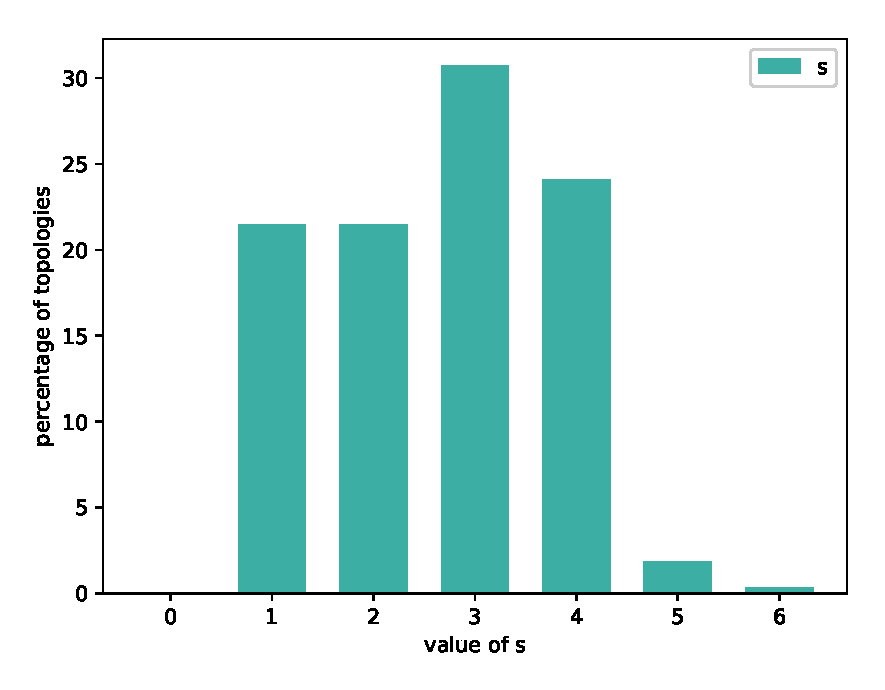
\includegraphics[width=.85\columnwidth]{./Network-lib/data/plot/primeIGP_s.eps}
\end{center}
\caption{Distribution, over all topologies, of the exponent $s$ required for $\igp^s$ to be ECMP-free and complete.}
\label{fig:primeIGP_s}
\end{figure}

We analyzed the percentage of topologies for which this process results in weights that go above the maximum configurable value $2^{16} - 1$.
It turns out that for this happens only for $2.3\%$ of the topologies as show in the CDF in Figure \ref{fig:primeIGP}. The threshold value
is shown with a dotted line.

\begin{figure}
\begin{center}
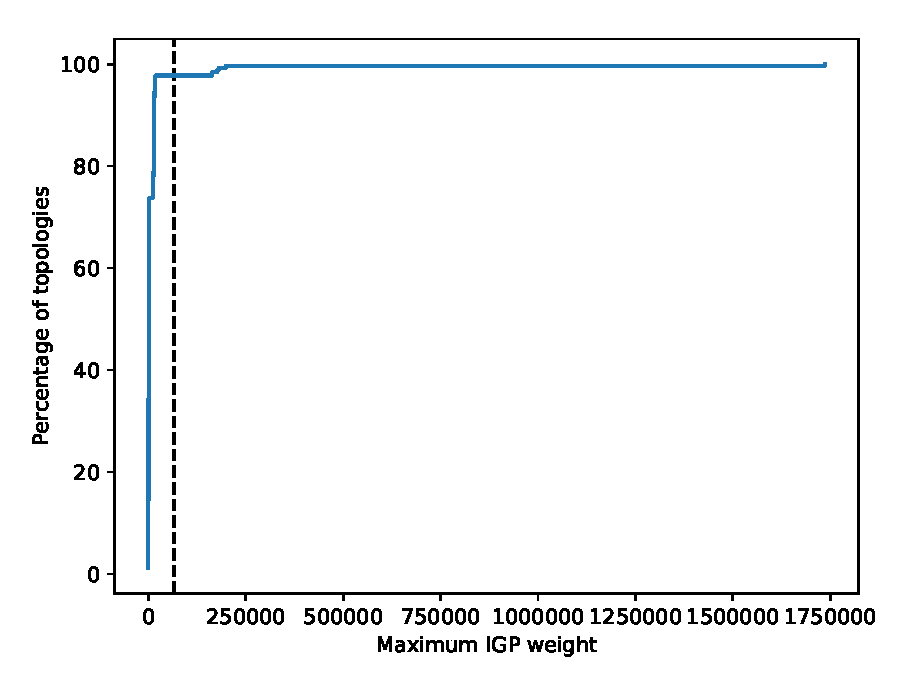
\includegraphics[width=.85\columnwidth]{./Network-lib/data/plot/primeIGP.eps}
\end{center}
\caption{CDF of maximum weight obtained over all topologies.}
\label{fig:primeIGP}
\end{figure}

Algorithm \ref{algo:primeIGP} provides a pseudo-code implementation of this algorithm described above.
The first step of the algorithm is to compute a set of $m = |E(G)|$ prime numbers. We can find these by iterating over the integers $2, 3, 5, 7, 9, \ldots$
and using any primality test algorithm to check which ones are prime numbers. The Prime number theorem \cite{Cormen:2009:IAT:1614191} %page 888 theorem 31.37
tells us that the $m$-th prime number is close to $m \cdot \ln(m)$ so we find them in a small number of steps.
This is not the most efficient way to achieve this but since $m$ is relatively small it is fast enough for our purposes.

\begin{algorithm}[t]
\small
\caption{$\textsf{primeIGP}\left( G \right)$}
\begin{algorithmic}[1]
%\algrule
\cmtline{compute the first $|E(G)|$ primes}
\STATE $m \gets |E(G)|$
\STATE $\mathcal{P} \gets \{ 2 \}$
\STATE $p \gets 3$
\WHILE{$|\mathcal{P}| < m$}
  \IF{$\textsf{isPrime}(p)$}
    \STATE $\mathcal{P} \gets \mathcal{P} \cup \{p\}$
  \ENDIF
  \STATE $p \gets p + 2$
\ENDWHILE
\cmtline{initialize weights}
\STATE $f \gets 1$
\FOR{$e \in E(G)$}
  \STATE $w(e) \gets \lfloor f \cdot \log(p_e) \rfloor + \lfloor f \cdot \log(p_m) \rfloor$
\ENDFOR
\cmtline{iterate until weights converge}
\WHILE{\textbf{not} $\textsf{ECMP-free}(w)$ \textbf{or not} $\textsf{complete}(w)$}
  \STATE $f \gets 10 \cdot f$
  \FOR{$e \in E(G)$}
    \STATE $w(e) \gets \lfloor f \cdot \log(p_e) \rfloor + \lfloor f \cdot \log(p_m) \rfloor$
  \ENDFOR
\ENDWHILE
\RETURN $w$
\end{algorithmic}
\label{algo:primeIGP}
\end{algorithm}

\subsection{Randomized complete IGP}

In practice, there seems to be a much simpler solution for generating relatively small ECMP-free and complete IGP weights.
We performed some experiments that showed that random weighs tend to be ECMP-free as long as the maximum value is not too small.
Therefore, a solution for generating ECMP-free weights that are also complete is to randomly generate weights for each edge 
and then adding the maximum generated weight to each edge to guarantee completeness. Algorithms \ref{algo:randomIGP} and \ref{algo:randomw}
formalize this process. Note that without the step of adding the maximum weight, our experiments showed that the algorithm
has a low probability of success. This is normal because otherwise there is no control over the weight of a single edge 
and so it can easily happen that it is assigned a high value making it impossible for it to belong to a shortest path.

\begin{algorithm}[t]
\small
\caption{$\textsf{randomIGP}\left( G, M \right)$}
\begin{algorithmic}[1]
%\algrule
\STATE $w \gets \textsf{random-w}(G, M)$
\WHILE{\textbf{not} $\textsf{ECMP-free}(w)$ \textbf{or not} $\textsf{complete}(w)$}
  \STATE $w \gets \textsf{random-w}(G, M)$ 
\ENDWHILE
\RETURN $w$
\end{algorithmic}
\label{algo:randomIGP}
\end{algorithm}

\begin{algorithm}[t]
\small
\caption{$\textsf{random-w}\left( G, M \right)$}
\begin{algorithmic}[1]
%\algrule
\FOR{$e \in E(G)$}
  \STATE $w(e) \gets \textsf{random}(1, \ldots, M)$
\ENDFOR
\FOR{$e \in E(G)$}
  \STATE $w'(e) \gets w(e) + \max_{e \in E(G)} w(e)$
\ENDFOR
\RETURN $w'$
\end{algorithmic}
\label{algo:randomw}
\end{algorithm}

In practice we tried it over all topologies with $M = 100$ for each of them we found a solution on average in at most $2$ iterations (over $100$ runs).
For this reason, in practice we strongly recommend using this simple algorithm. However we were unable to prove any bound on the probability of success
of this algorithm. Hence we cannot say whether it will work well beyond our dataset. We leave the following problem as another interesting open problem.

\begin{lemma}
For any network $G$ and $M \in \mathbb{N}$ the weight function produced by Algorithm \ref{algo:randomw} is complete. 
\end{lemma}

\begin{proof}
Let $w$ be the random weights produced by the algorithm after the first loop and $w'$ the final weights. Let $M = \max_{e \in E(G)} w(e)$. 
Let $u, v \in V(G)$ and $p$ be a path from $u$ to $v$ with at least two edges.
Then
$$
w'(p) = w(p) + |E(p)| \cdot M > 2 \cdot M \geq w(e) + M = w'(e)
$$
for any edge $e \in E(G)$. Therefore the shortest path between $u$ and $v$ must be a single edge $e \in E(G, u, v)$.
\end{proof}

\begin{problem}{Randomized weighting}
\label{prob:randomIGP}
\textbf{Input:} A network $G$ and a integer constant $M \in \mathbb{N}$. 

\textbf{Output:} The probability that $\textsf{random-w}\left( G, M \right)$ outputs an ECMP-free IGP weight function.
\end{problem}

\subsection{Cycle covers with ECMP-free and complete IGP}

In this section we evaluate the benefits of using ECMP-free and complete IGP weights.
We start by evaluating the minimum number of segments required in a minimum segment cost
sr-cycle cover. Recall that Algorithm \ref{algo:min-seg-cover2} computes a sr-cycle cover such
that the maximum number of segments in any sr-cycle is as small as possible. In Figure 
\ref{fig:min-seg-cover-segcost} we already evaluated the segment cost of the solutions obtained 
by this algorithm over the original IGP weights. Figure \ref{fig:min-seg-cost-segcost-new} shows
the distribution of the segment costs with and without special IGP weights. We observe that ECMP-free
and complete weights obtain the desired effect of greatly reducing the segment cost of minimum
cost sr-cycle covers. For $100\%$ of the topologies we need sr-cycles with segment cost at most $4$ whereas before
about $55\%$ of the topologies required sr-cycles with segment cost $5$ or more.

\begin{figure}
\begin{center}
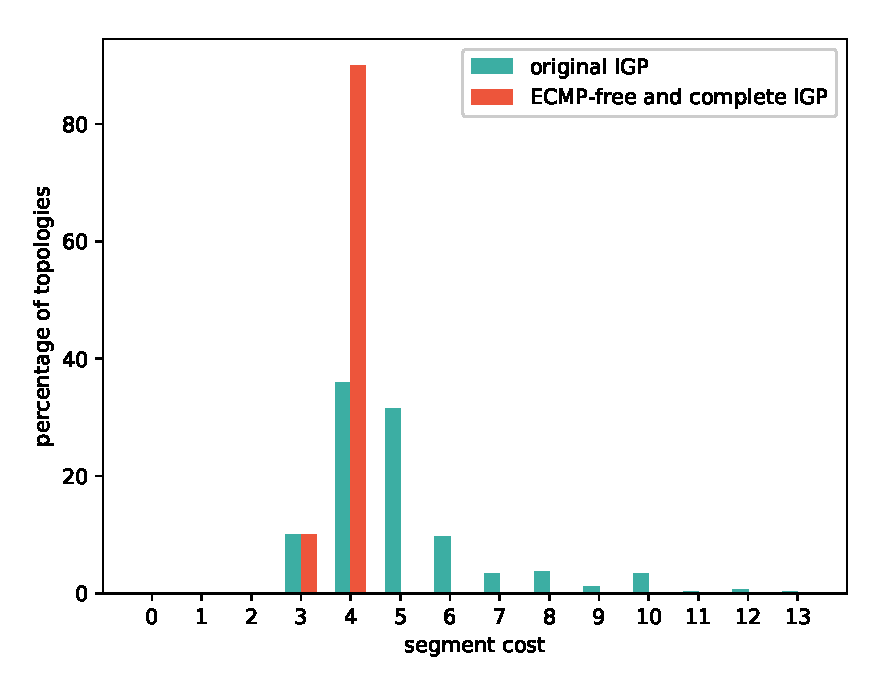
\includegraphics[width=.85\columnwidth]{./Network-lib/data/plot/minSegCover_segcost_complete.eps}
\end{center}
\caption{Distribution of the maximum segment cost of the probing sr-cycles with and without ECMP-free and complete weights.}
\label{fig:min-seg-cost-segcost-new}
\end{figure}

Next we analyze the benefits of using special IGP weights with respect to the segment cost of the 
identification sr-cycles. Recall that our network monitoring solution uses probing sr-cycles to periodically
check whether every link is still up and one identification sr-cycles to pinpoint a failure when
a monitoring probe fails to return to the vantage point. Figure \ref{fig:min-seg-cost-segcost-new}
shows how much do we gain in terms of segment cost by having ECMP-free and complete IGP weights. We can see that
using these weights makes it possible to implement such a monitoring scheme on a lot more networks since the maximum
number of segments required becomes $9$ rather than the original high value of $19$.

\begin{figure}
\begin{center}
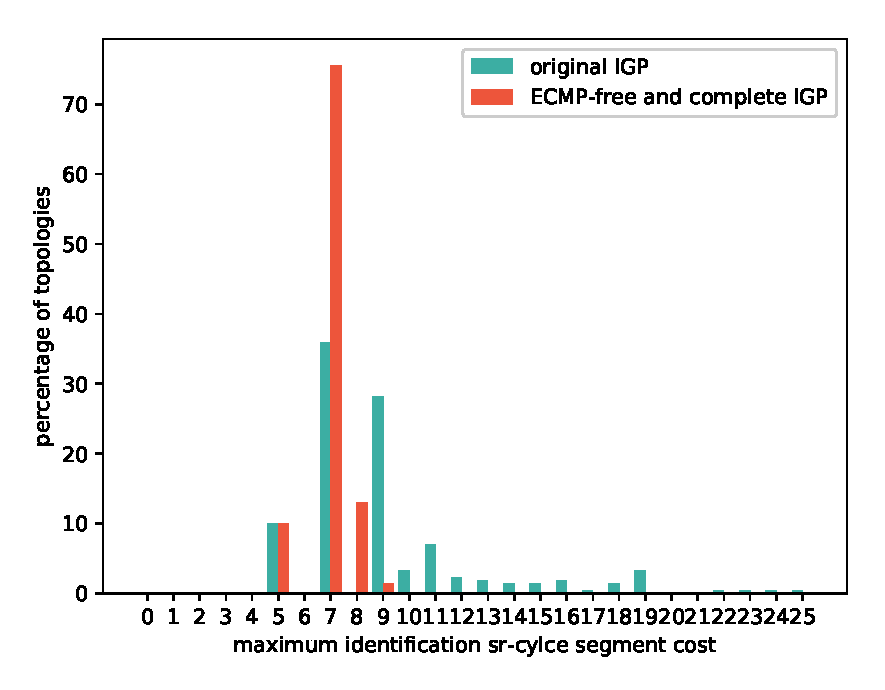
\includegraphics[width=.85\columnwidth]{./Network-lib/data/plot/minSegCover_identification.eps}
\end{center}
\caption{Distribution of the maximum segment cost of the identification sr-cycles with and without ECMP-free and complete weights.}
\label{fig:min-seg-cost-segcost-new}
\end{figure}
